\section{PCA}

\begin{frame}%[allowframebreaks]
  \frametitle{Redução de Dimensionalidade}
  \begin{itemize}
  \item Aprendizado de máquina (Machine Learning)
  \item reduzir o número de variáveis aleatórias que são consideradas em um problema
  \item seleção de características
  \item extração de características
  \item visualização dos dados
  \item evitar a maldição da dimensionalidade
  \end{itemize}  
\end{frame}
\note{
Quando o número de dimensões cresce, o volume do espaço onde estão os dados cresce rapidamente, de forma
que os dados tornam-se esparsos. Isto torna-se um problema para muitos métodos que requerem uma significância
estatística. Para obter um resultado estatisticamente confiável, a quantidade de dados necessária para
embasar o resultado geralmente cresce exponencialmente com o número de dimensões do problema.
Além disso, organizar e buscar dados usualmente depende da detecção de áreas onde os objetos formam
grupos com propriedades similares; quando os dados possuem um grande número de dimensões, todos os
objetos parece esparsos e dissimilares, o que não permite que as estratégias de organização de dados sejam
eficientes.
}

\begin{frame}%[allowframebreaks]
  \frametitle{Principal Component Analysis (PCA)}
  A PCA é uma transformação linear que realiza um mapeamento dos dados para um espaço em que a maior parte
  da variância dos dados está concentrada em poucas dimensões. Desta forma é possível selecionar apenas 
  algumas dimensões, mantendo a variância dos dados.  
\end{frame}

\begin{frame}%[allowframebreaks]
  \frametitle{PCA - exemplo}
  \begin{figure}[h!]
  \centering
  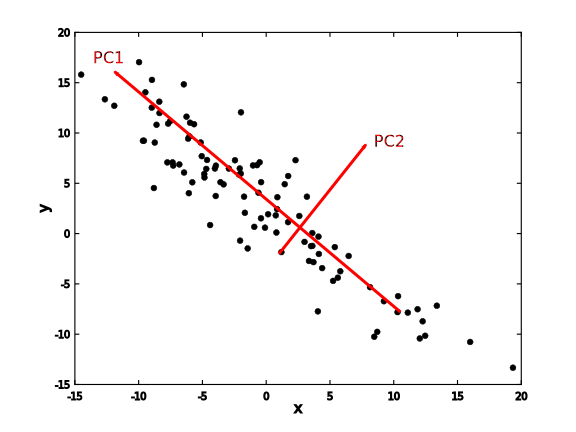
\includegraphics[width=0.5\textwidth]{images/pca_ex1.pdf}
  \caption{Exemplo PCA.}
  \label{fig:pcaex1}
  \end{figure}  
\end{frame}
% x(1,:) = 2 + 2*randn(1,100);
% x(2,:) = 2 + 10*randn(1,100);
% R = [cos(pi/4) -sin(pi/4); sin(pi/4) cos(pi/4)];
% y = R*x;
% plot(y(1,:),y(2,:),'ko'); xlabel ('x'); ylabel ('y');

\begin{frame}%[allowframebreaks]
  \frametitle{PCA - exemplo}
  \begin{figure}[h!]
  \centering
  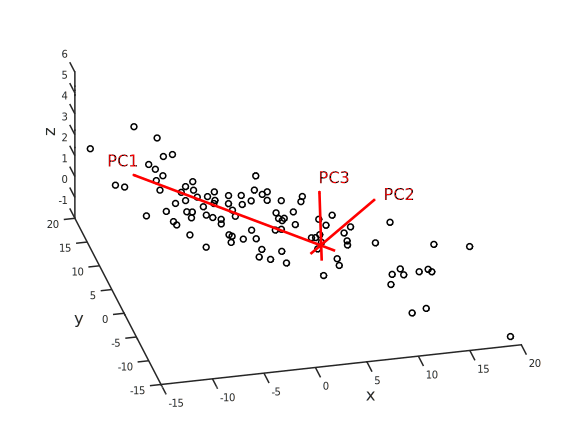
\includegraphics[width=0.5\textwidth]{images/pca_ex2.pdf}
  \caption{Exemplo PCA.}
  \label{fig:pcaex2}
  \end{figure}  
\end{frame}

\begin{frame}%[allowframebreaks]
  \frametitle{PCA - exemplo}
  \begin{figure}[h!]
  \centering
  \includegraphics[width=0.5\textwidth]{images/twos.jpg}
  \caption{Fonte: \url{http://web.mit.edu/cocosci/isomap/datasets.html}}
  \label{fig:twos}
  \end{figure}
\end{frame}

\begin{frame}%[allowframebreaks]
  \frametitle{PCA - exemplo}
  \begin{figure}[h!]
  \centering
  \includegraphics[width=0.8\textwidth]{images/nonlinear.jpg}
  \caption{\emph{kernel} PCA - aplicar uma transformação não-linear anterior à PCA.}
  \label{fig:nonlinear}
  \end{figure}
\end{frame}


\begin{frame}%[allowframebreaks]
  \frametitle{PCA vs Regressão Linear}
  \begin{figure}[h!]
  \centering
  \includegraphics[width=0.4\textwidth]{images/pcavsfit.png}
  \caption{PCA vs Regressão Linear. \url{https://stackoverflow.com/questions/8457279/visual-comparison-of-regression-pca}}
  \label{fig:pcavsfit}
  \end{figure} 
\end{frame}
\note{
Na regressão linear teremos $y$ como uma função de $x$, e desta forma iremos procurar a reta que 
fornece a melhor predição (menor erro: $e = y - \hat{y}$).

Na PCA iremos encontrar a dimensão sob a qual teremos o menor erro ao realizar a projeção 
(erro $e = \vert\vert \mathbf{p_i} - \mathbf{p_i}^{\textmd{pca}} \vert\vert$).
%(erro $e = \vert\vert \mathbf{p_i} - \mathbf{p_i}^\textmd{pca}  \vert\vert$).
}


\begin{frame}[allowframebreaks]
  \frametitle{Pré-Processamento}  
  Dados de treinamento: $x^{(1)}, x^{(2)}, \ldots, x^{(m)}$.

  Pré-processamento (escalonamento de cada característica / normalização da média)

  Normalização da média:
  \begin{itemize}
  \item calcular a média de cada característica
  \begin{equation}
  \mu_j = \frac{1}{m} \sum_{i=1}^{m} x_{j}^{(i)}
  \end{equation}
  \item substituir cada $x_{j}^{(i)}$ por $x_{j}^{(i)} - \mu_{j}$.
  \end{itemize}

  \framebreak

  Cada característica (dimensão) possui uma escala diferente. É necessário realizar uma mudança de escala
  para que os valores apresentem extensões similares e uma característica não domine outra.
  \begin{itemize}
  \item realizar a seguinte substituição
  \begin{equation}
  x_{j}^{(i)} \leftarrow \frac{ x_{j}^{(i)} - \mu_{j} }{\sigma_j}
  \end{equation}
  \end{itemize}

\end{frame}

\begin{frame}%[allowframebreaks]
  \frametitle{PCA - algoritmo} 
  \begin{enumerate}
  \item realizar o pré-processamento, se necessário
  \item calcular a matriz de covariância dos dados
  \item encontrar os autovetores da matriz de covariância (utilizar a decomposição em valores singulares)
  \end{enumerate}   
\end{frame}

\subsection{Dados}
\begin{frame}[allowframebreaks]
  \frametitle{Dataset}
  
  Nosso conjunto de dados possui $n$ amostras.
  
  Cada amostra $\mathbf{x}^{(i)}$ é um vetor em um espaçado de $m$ dimensões, $\mathbf{x}^{(i)} \in \mathbb{R}^m$.
  \begin{equation}
  \mathbf{x}^{(i)} = [x_1^{(i)}, x_2^{(i)}, \ldots, x_m^{(i)}]^T
  \end{equation}
  
  Podemos representar os dados por uma matriz $m \times n$, onde cada coluna é uma amostra $\mathbf{x}^{(i)}$.
  
  \begin{equation}
  \mathbb{X} = \begin{bmatrix} \mathbf{x}^{(1)} & \mathbf{x}^{(2)} & \ldots & \mathbf{x}^{(n)} \end{bmatrix}  = 
  \begin{bmatrix}
  x_{1}^{(1)} & x_{1}^{(2)} & \ldots & x_{1}^{(n)} \\
  x_{2}^{(1)} & x_{2}^{(2)} & \ldots & x_{2}^{(n)} \\
  \vdots  & \vdots  & \ddots & \vdots  \\
  x_{m}^{(1)} & x_{m}^{(2)} & \ldots & x_{m}^{(n)}
  \end{bmatrix}  
  \end{equation}
 
  \framebreak
  
  \begin{equation}
  \mathbb{X} = \begin{bmatrix} \mathbf{x}^{(1)} & \mathbf{x}^{(2)} & \ldots & \mathbf{x}^{(n)} \end{bmatrix}  = 
  \begin{bmatrix}
  x_{1,1} & x_{1,2} & \ldots & x_{1,n} \\
  x_{2,1} & x_{2,2} & \ldots & x_{2,n} \\
  \vdots  & \vdots  & \ddots & \vdots  \\
  x_{m,1} & x_{m,2} & \ldots & x_{m,n}
  \end{bmatrix}  
  \end{equation}

  Elemento $x_{i,j} = x_{i}^{(j)}$, $i$-ésima característica do $j$-ésima amostra.
\end{frame}

\subsection{Covariância}
\begin{frame}[allowframebreaks]
  \frametitle{Mudança de Base}
  
  Desejamos realizar uma mudança de base.

  \begin{itemize}
  \item Existe uma outra base, que seja uma combinação linear da base original, que melhor represente os nossos dados?
  \end{itemize}   

  \vspace{0.5cm}
  Transformação linear (rotação e estiramento): $\mathbf{P}$. \\
  Dados originais: $\mathbf{X}$. \\
  Após a transformação: $\mathbf{Y}$. \\

  \begin{equation}
  \mathbf{Y} = \mathbf{P} \mathbf{X}
  \end{equation}

  \framebreak

  As linhas de $\mathbf{P}$ são os vetores base para a representação dos dados nas colunas de $\mathbf{X}$.

  \begin{equation}
  \mathbf{P} \mathbf{X} = \begin{bmatrix} \mathbf{p_1} \\ \vdots \\ \mathbf{p_m} \end{bmatrix} \begin{bmatrix} \mathbf{x_1} & \ldots & \mathbf{x_n} \end{bmatrix}
  \end{equation}

  \begin{equation}
  \mathbf{Y} = 
  \begin{bmatrix} 
  \mathbf{p_1} \cdot \mathbf{x_1} & \ldots & \mathbf{p_1} \cdot \mathbf{x_n} \\
  \vdots & \ddots & \vdots \\
  \mathbf{p_m} \cdot \mathbf{x_1} & \ldots & \mathbf{p_m} \cdot \mathbf{x_n}
  \end{bmatrix}
  \end{equation}

  \framebreak

  Cada coluna de $\mathbf{Y}$ é da forma
  \begin{equation}
  \mathbf{y_i} = \begin{bmatrix} \mathbf{p_1} \cdot \mathbf{x_i} \\ \vdots \\ \mathbf{p_m} \cdot \mathbf{x_i} \end{bmatrix}
  \end{equation}

  Observamos que cada coeficiente de $\mathbf{y_i}$ é o produto interno entre $\mathbf{x_i}$ e a linha correspondente de $\mathbf{P}$, ou seja,
  o $j$-ésimo coeficiente de $\mathbf{y_i}$ é a projeção de $\mathbf{x_i}$ na $j$-ésima linha de $\mathbf{P}$.

\end{frame}

\begin{frame}[allowframebreaks]
  \frametitle{Variância e Objetivo}
  Qual é a melhor base na qual queremos representar nossos dados? Como escolher $\mathbf{P}$?

  \begin{itemize}
  \item ruido deve ser baixo (alta relação sinal-ruido)
  \begin{equation}
  \textmd{SNR} = \frac{\sigma^2_{\textmd{sinal}}}{\sigma^2_{\textmd{ruido}}}
  \end{equation}
  \end{itemize}
  \vspace{-0.25cm}
  \begin{figure}[h!]
  \centering
  \includegraphics[width=0.3\textwidth]{images/snr.png}
  \caption{Relação sinal ruído \citep{shlens2014}.}
  \label{fig:snr}
  \end{figure}

  \framebreak

  \begin{itemize}
  \item redundância
  \end{itemize}

  $r_1$ e $r_2$ são duas medições arbitrárias 
  \begin{figure}[h!]
  \centering
  \includegraphics[width=0.4\textwidth]{images/redundancy.png}
  \caption{Redundância \citep{shlens2014}.}
  \label{fig:redundancy}
  \end{figure}
 
\end{frame}

\begin{frame}%[allowframebreaks]
  \frametitle{Variância e Objetivo}
  \begin{figure}[h!]
  \centering
  \includegraphics[width=0.55\textwidth]{images/toy-ex.png}
  \caption{Exemplo hipotético \citep{shlens2014}.}
  \label{fig:toy-ex}
  \end{figure}
  \vspace{-0.5cm}
  \begin{small}
  Neste exemplo temos medições provenientes de 3 câmeras diferentes, com orientações distintas.
  Cada uma belas observa a movimentação do objeto através de uma projeção em duas dimensões,
  Entretanto, sabemos que o objeto movimenta-se ao longo de uma única dimensão.
  \end{small}
\end{frame} 

\begin{frame}[allowframebreaks]
  \frametitle{Matriz de Variância}
  A SNR é calculada pela variância.

  Considere os conjuntos de medição com média nula
  \begin{equation}
  A = \{ a_1 , a_2 , \ldots , a_n \} \ \textmd{ e } \ B = \{ b_1, b_2 , \ldots , b_n\}
  \end{equation}

  A variância é dada
  \begin{equation}
  \sigma_A^2 = \langle a_i a_i \rangle_i   \ \textmd{ e } \  \sigma_B^2 = \langle b_i b_i \rangle_i
  \end{equation}
  onde o valor esperado é a média sobre $n$ variáveis.

  O valor esperado $\langle \cdot \rangle_i$ é denotado pela média sobre valores indexados por $i$,
  pois a média é nula.
  $\sigma_X = E[(X-\mu_X)(X-\mu_X)]$

  \framebreak 

  A covariância entre $A$ e $B$ é dada por
  \begin{equation}
  \sigma_{AB}^2 = \langle a_i b_i \rangle_i
  \end{equation}

  \begin{itemize}
  \item $\sigma_{AB}^2 = 0$ se e somente se $A$ e $B$ são inteiramente descorrelacionados
  \item $\sigma_{AB}^2 = \sigma_{A}^2$ se $A=B$
  \end{itemize}

\end{frame}


\begin{frame}[allowframebreaks]
  \frametitle{Variância}
  Representando na forma vetorial.

  \begin{equation}
  \mathbf{a} = \begin{bmatrix} a_1 & a_2 & \ldots & a_n \end{bmatrix}
  \end{equation}

  \begin{equation}
  \mathbf{b} = \begin{bmatrix} b_1 & b_2 & \ldots & b_n \end{bmatrix}
  \end{equation}


  \begin{equation}
  \sigma_{\mathbf{ab}}^2 \equiv \frac{1}{n-1} \mathbf{ab}^T
  \end{equation}
  onde o primeiro termo é a constante de normalização\footnote{A normalização mais
  simples é utilizando $\frac{1}{n}$, entretanto, desta forma teríamos um estimador
  polarizado para a variância, particularmente para $n$ pequeno. Para obter um estimador
  não polarizado para a variância, devemos utilizar $\frac{1}{n-1}$.}.

\end{frame} 

\begin{frame}[allowframebreaks]
  \frametitle{Matriz de Covariância}

  \begin{equation}
  \mathbf{X} = \begin{bmatrix} \mathbf{x_1} \\ \vdots \\ \mathbf{x_m} \end{bmatrix}
  \end{equation}

  Cada linha de $\mathbf{X}$ representa uma amostra (conjuntos de medições/características de um tipo).

  A matriz de covariância é definida então
  \begin{equation}
  \mathbf{S_X} \equiv \frac{1}{n-1} \mathbf{X} \mathbf{X}^T
  \end{equation}

  \begin{itemize}
  \item $\mathbf{S_X}$ é uma matriz quadrada simétrica $m \times m$
  \item os valores na diagonal de $\mathbf{S_X}$ são a variância de uma medição (uma amostra)
  \item os valores fora da diagonal são valores de covariância entre duas medições (amostras) distintas 
  \end{itemize}
\end{frame}



\begin{frame}[allowframebreaks]
  \frametitle{Diagonalização da Matriz de Covariância}

  Queremos reduzir a redundância, ou seja, queremos que cada variável co-varie o mínimo possível uma com as outras.
  
  O objetivo então é encontrar $\mathbf{Y}$ de forma que $\mathbf{S_Y}$ seja uma matriz diagonal.

  \begin{itemize}
  \item existem diversas formas de diagonalizar $\mathbf{S_Y}$
  \item PCA é uma dessas forma. A PCA assume que os vetores de base $\{\mathbf{p_1}, \ldots , \mathbf{p_m} \}$ são ortonormais
  \item a PCA utilizará uma matriz ortonormal $\mathbf{P}$
  \end{itemize}

\end{frame}

\begin{frame}[allowframebreaks]
  \frametitle{Autovetores da Covariância}
  \begin{itemize}
  \item Desejamos encontrar uma matriz ortonormal $\mathbf{P}$, onde $\mathbf{Y} = \mathbf{P} \mathbf{X}$ esteja sujeito a $\mathbf{S_Y} \equiv \frac{1}{n-1} \mathbf{Y} \mathbf{Y}^T$ ser uma matriz diagonal. As linhas de $\mathbf{P}$ são as componentes principais de $\mathbf{X}$.
  \end{itemize}


\begin{eqnarray}
\mathbf{S_Y} &=& \frac{1}{n-1} \mathbf{Y} \mathbf{Y}^T \nonumber \\
             &=& \frac{1}{n-1} (\mathbf{P} \mathbf{X})(\mathbf{P} \mathbf{X})^T \nonumber \\
             &=& \frac{1}{n-1} \mathbf{P} (\mathbf{X} \mathbf{X}^T) \mathbf{P}^T \nonumber \\
             &=& \frac{1}{n-1} \mathbf{P} \mathbf{A} \mathbf{P}^T 
\end{eqnarray}

Definimos a matriz simétrica $\mathbf{A} \equiv \mathbf{X} \mathbf{X}^T$.
\end{frame} 

\begin{frame}[allowframebreaks]
  \frametitle{Diagonalização - teorema 1}
  Serão utilizados dois teoremas.
  % teorema 3 e 4

  \begin{block}{uma matriz é simétrica se e somente se é ortogonalmente diagonalizável}
  \begin{enumerate}
  \item Se $\mathbf{A}$ é uma matriz ortogonalmente diagonalizável, então, por hipótese, exite $\mathbf{E}$ tal que $\mathbf{A} = \mathbf{E} \mathbf{D} \mathbf{E}^T$, onde $\mathbf{D}$ é diagonal. Desta forma, teremos
  \begin{equation}
  \mathbf{A}^T = (\mathbf{E} \mathbf{D} \mathbf{E}^T)^T = \mathbf{E}^{TT} \mathbf{D}^T \mathbf{E}^T = \mathbf{E} \mathbf{D} \mathbf{E}^T = \mathbf{A}
  \end{equation}
  e concluímos que a matriz $\mathbf{A}$ é simétrica.
  \item mostrar que: Se uma matriz $\mathbf{A}$ é simétrica, então ela será ortogonalmente diagonalizável.
  \end{enumerate}
  \end{block}
\end{frame}

\begin{frame}[allowframebreaks]
  \frametitle{Diagonalização - teorema 2}
  \begin{block}{uma matriz simétrica é diagonalizada pela matriz de seus autovetores ortonormais}
  Seja $\mathbf{A}$ uma matriz simétrica $n \times n$ com autovetores associados $\{ \mathbf{e_1}, \mathbf{e_2}, \ldots, \mathbf{e_n} \}$.
  Seja $\mathbf{E}$ tal que cada $i$-ésima coluna é um autovetor $\mathbf{e_i}$ de $\mathbf{A}$, então $\mathbf{E} = \begin{bmatrix} \mathbf{e_1} & \mathbf{e_2} & \ldots & \mathbf{e_n} \end{bmatrix}$.
  Então existe uma matriz diagonal $\mathbf{D}$ tal que $\mathbf{A} = \mathbf{E}\mathbf{D}\mathbf{E}^T$.

  Demonstração em duas partes:
  \begin{enumerate}
  \item qualquer matriz pode ser ortogonalmente diagonalizável se e somente se os autovetores desta matriz forem linearmente independentes
  \item uma matriz simétrica possui autovetores que são ortogonais
  \end{enumerate}
  \end{block}
\end{frame}

\begin{frame}[allowframebreaks]
  \frametitle{Diagonalização - teorema 2 - parte 1}

  Seja $\mathbf{A}$ uma matriz qualquer e $\mathbf{E} = \begin{bmatrix} \mathbf{e_1} & \mathbf{e_2} & \ldots & \mathbf{e_n} \end{bmatrix}$ a matriz de autovetores de $\mathbf{A}$.
  Vamos criar uma matriz $\mathbf{D}$ em que o $i$-ésimo autovalor de $\mathbf{A}$ seja colocado na posição $(i,i)$ da matriz $\mathbf{D}$. Pela definição de autovalor e autovetor, temos
  \begin{equation}
  \mathbf{A} \mathbf{e_i} = \lambda_i \mathbf{e_i}
  \end{equation}
  Desta forma, podemos escrever
  \begin{eqnarray}
  \begin{bmatrix} \mathbf{A} \mathbf{e_1} & \mathbf{A} \mathbf{e_2} & \ldots & \mathbf{A} \mathbf{e_n} \end{bmatrix} &=& \begin{bmatrix} \lambda_1 \mathbf{e_1} & \lambda_2 \mathbf{e_2} & \ldots & \lambda_n \mathbf{e_n} \end{bmatrix} \nonumber \\ 
  \mathbf{A} \mathbf{E} &=& \mathbf{E} \mathbf{D}
  \end{eqnarray}
  e assim teremos
  \begin{equation}
  \mathbf{A} = \mathbf{E} \mathbf{D} \mathbf{E}^{-1}
  \end{equation}
\end{frame}

\begin{frame}[allowframebreaks]
  \frametitle{Diagonalização - teorema 2 - parte 2}
  Uma matriz simétrica sempre possui autovetores ortogonais.

  Sejam $\lambda_1$ e $\lambda_2$ autovalores distintos de autovetores $\mathbf{e_1}$ e $\mathbf{e_2}$.
  \begin{eqnarray}
  \lambda_1 \mathbf{e_1} \cdot \mathbf{e_2} &=& (\lambda_1 \mathbf{e_1})^T \mathbf{e_2} \nonumber \\
                                            &=& \left( \mathbf{A} \mathbf{e_1}\right)^T \mathbf{e_2} \nonumber \\
                                            &=& \mathbf{e_1}^T \mathbf{A}^T \mathbf{e_2} \nonumber \\
                                            &=& \mathbf{e_1}^T \mathbf{A} \mathbf{e_2} \nonumber \\
                                            &=& \mathbf{e_1}^T (\lambda_2 \mathbf{e_2}) \nonumber \\
                                            &=& \lambda_2 \mathbf{e_1} \cdot \mathbf{e_2}
  \end{eqnarray}
  Concluímos que $(\lambda_1 - \lambda_2) \mathbf{e_1} \cdot \mathbf{e_2} = 0$. Como os autovalores são únicos,
  deveremos ter $\mathbf{e_1} \cdot \mathbf{e_2} = 0$. Desta forma, os autovetores de uma matriz simétrica são ortogonais.
\end{frame} 
\note{
Um autovetor multiplicado por um escalar será também autovetor. Logo, por definição iremos
escolher autovetores com norma unitária, assim podemos afirmar que os autovetores de uma
matriz simétrica são ortonormais.
}

\begin{frame}[allowframebreaks]
  \frametitle{Diagonalização - teorema 2}
  Como $\mathbf{E}$ é uma matriz ortogonal, teremos $\mathbf{E}^{T} = \mathbf{E}^{-1}$ e, desta forma,

  \begin{equation}
  \mathbf{A} = \mathbf{E} \mathbf{D} \mathbf{E}^{T}
  \end{equation}

  Uma matriz simétrica é diagonalizável por uma matriz de seus autovetores.
\end{frame}
 
\begin{frame}[allowframebreaks]
  \frametitle{Diagonalização}
  A matriz de autocorrelação é simétrica e poderá portanto ser decomposta como
  \begin{equation}
  \mathbf{A} = \mathbf{E} \mathbf{D} \mathbf{E}^{T}
  \end{equation}
  onde $\mathbf{D}$ é uma matriz diagonal e $\mathbf{E}$ é a matriz de autovetores de $\mathbf{A}$.


  \begin{itemize}
  \item a matriz $\mathbf{A}$ possui $r \leq m$ autovetores ortonormais, onde $r$ é o posto da matriz.
  \end{itemize}  
\end{frame}
\note{
O posto de $\mathbf{A}$ é menor do que $m$ quando $\mathbf{A}$ é degenerada, ou quando todos os dados ocupam um subespaço de dimensão $r \leq m$.
Para remediar este empecilho, podemos adicionar outros $(m-r)$ vetores ortonormais para preencher a matriz $\mathbf{E}$. Estes vetores não
terão efeito na solução final pois a variância associada a eles será nula.

O posto de uma matriz $\mathbf{A}$ é o número de linhas ou colunas linearmente independentes de $\mathbf{A}$,
ou equivalentemente, é o número de linhas não-nulas quando a mesma está escrita na forma reduzida escalonada por linhas. 
}

\begin{frame}[allowframebreaks]
  \frametitle{Diagonalização}
  Vamos selecionar a matriz $\mathbf{P}$ de forma que cada linha $\mathbf{p_i}$ seja um autovetor de $\mathbf{X}\mathbf{X}^T$, ou seja, $\mathbf{P} \equiv \mathbf{E}^T$.
  Teremos então
  \begin{eqnarray}
  \mathbf{S_Y} &=& \frac{1}{n-1} \mathbf{P} \mathbf{A} \mathbf{P}^T \nonumber \\
               &=& \frac{1}{n-1} \mathbf{P} (\mathbf{P}^T \mathbf{D} \mathbf{P} ) \mathbf{P}^T  \nonumber \\
               &=& \frac{1}{n-1} (\mathbf{P} \mathbf{P}^T) \mathbf{D} (\mathbf{P} \mathbf{P}^T) \nonumber \\
               &=& \frac{1}{n-1} (\mathbf{P} \mathbf{P}^{-1}) \mathbf{D} (\mathbf{P} \mathbf{P}^{-1}) \nonumber \\
               &=& \frac{1}{n-1} \mathbf{D}
  \end{eqnarray}
  Fica assim evidente que a escolha feita para $\mathbf{P}$ diagonaliza a matriz $\mathbf{S_Y}$, o que é o objetivo da PCA. 
\end{frame}

\begin{frame}[allowframebreaks]
  \frametitle{Resultado da PCA}
  Como resultado da PCA teremos
  \begin{itemize}
  \item as componentes principais de $\mathbf{X}$ são autovetores de $\mathbf{X}\mathbf{X}^T$; que serão linhas de $\mathbf{P}$.
  \item o $i$-ésimo valor na diagonal de $\mathbf{S_Y}$ representa a variância de $\mathbf{X}$ ao longo da direção de $\mathbf{p_i}$.
  \end{itemize}
\end{frame}

\begin{frame}%[allowframebreaks]
  \frametitle{Notebook - PCA}
  \centering
  \includegraphics[width=0.4\textwidth]{images/qrcode-jupyter-pca.pdf}

  \url{https://nbviewer.jupyter.org/github/leolca/notebooks/blob/master/aev/pca.ipynb}
\end{frame} 
